\chapter{Classi concrete}
\section{Classi concrete sviluppate}
\begin{itemize}
	\item Classi utilizzate per l'\textbf{input}:
	\begin{enumerate}
		\item Sonar.cpp, Sonar.h;
		\item Button.cpp, Button.h.
	\end{enumerate}
	\item Classi utilizzate per l'\textbf{output}:
	\begin{enumerate}
		\item Buzzer.cpp, Buzzer.h;
		\item Led.cpp, Led.h;
		\item LedPwm.cpp, LedPwm.h;
		\item LedRgb.cpp, LedRgb.h;
		\item MessageService.cpp, MessageService.h;
		\item Multiplexer.cpp, Multiplexer.h.
	\end{enumerate}
	\item Classi utilizzate per coordinare il \textbf{multi-tasking}:
	\begin{enumerate}
		\item Context.h;
		\item Scheduler.cpp, Scheduler.h;
		\item Timer.h, Timer.cpp;
		\item Tash.h.
	\end{enumerate}
	\item Classi dei \textbf{task}:
	\begin{enumerate}
		\item ButtonTask.cpp, ButtonTask.h;
		\item BuzzerTask.cpp, BuzzerTask.h;
		\item LedPwmTask.cpp, LedPwmTask.h;
		\item LedRgbTask.cpp, LedRgbTask.h;
		\item LedTask.cpp, LedTask.h;
		\item SonarTask.cpp, SonarTask.h.
	\end{enumerate}
\end{itemize}

\section{Gestione dell'input}
\subsection{Sonar.cpp, Sonar.h}
Questa classe permette di leggere la distanza tra la mano del giocatore ed il sensore ad ultrasuoni.

Per ottenere un input molto performante dal punto di vista del tempo e dell'accuratezza, è stata sfruttata la libreria \href{http://playground.arduino.cc/Code/NewPing}{NewPing}.

In particolare nel costruttore di Sonar viene istanziato un oggetto \texttt{NewPing} a cui sono passati tre parametri:
\begin{itemize}
	\item \texttt{trigPin}: pin settato come output a cui è fisicamente collegato il trigger del sonar;
	\item \texttt{echoPin}: pin settato come output a cui è fisicamente collegato l'echo del sonar;
	\item \texttt{maxDistance}: limita massimo di distanza gestito oltre il quale la mano non viene rilevata e non si possono creare lucchetti.
\end{itemize}
\subsubsection{Metodi}
\begin{itemize}
	\item \texttt{int readDistance()}: lettura istantanea della distanza sensore-mano espressa in cm.
\end{itemize}
\begin{figure}[!ht]
	\centering
	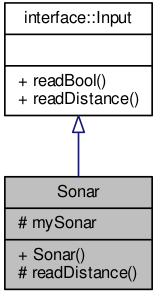
\includegraphics[scale=.5]{img/UML/CollaborationDiagram/Sonar.png}
	\caption{Collaboration Diagram - Sonar}
\end{figure}
\begin{figure}[!ht]
	\centering
	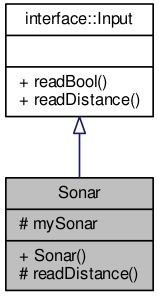
\includegraphics[scale=.5]{img/UML/InheritanceDiagram/Sonar.png}
	\caption{Inheritance Diagram - Sonar}
\end{figure}

\newpage
\subsection{Button.cpp, Button.h}
Anche questa classe implementa l'interfaccia Input. Lo scopo è riconoscere la pressione del button, evitando gli effetti del floating.

Il pin è stato configurato come \textit{INPUT\_PULLUP} in modo da sfruttare la resistenza interna dell'Arduino, ottenendo:
\begin{itemize}
	\item dei campionamenti con un rumori ridotti;
	\item floating del button quasi annullato.\footnote{Questa scelta di progetto è confermata dal tutorial: \href{http://tinyurl.com/jqp8nwu}{Arduino Internal Pull-Up Resistor}.}
\end{itemize}

\subsubsection{Metodi}
\begin{itemize}
	\item \texttt{bool readBool()}: prende come input il valore del pin disposto in configurazione INPUT\_PULLUP e lo nega. Se tale valore è falso viene campionato il tempo attuale. Se al successivo cambio di stato non è passato un tempo fissato e considerato sicuro, per evitare involontari cambi di stato, viene ignorato il segnale.
\end{itemize}
\begin{figure}[!ht]
	\centering
	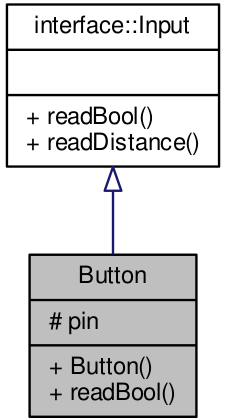
\includegraphics[scale=.35]{img/UML/CollaborationDiagram/Button.png}
	\caption{Collaboration Diagram - Button}
\end{figure}
\begin{figure}[!ht]
	\centering
	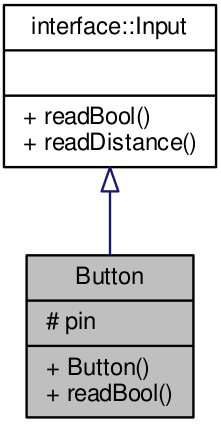
\includegraphics[scale=.35]{img/UML/InheritanceDiagram/Button.png}
	\caption{Inheritance Diagram - Button}
\end{figure}

\newpage
\section{Gestione dell'output}
\subsection{Buzzer.cpp, Buzzer.h}
Questa classe gestisce il buzzer, permettendo emettere dei suoni. Nel progetto è stato utile per far comprendere al giocatore lo stato di scasso del lucchetto.
\subsubsection{Metodi}
\begin{itemize}
	\item \texttt{public void playSound(const int sound)}: in base al numero intero passato a questo metodo, viene configurato il suono che il buzzer deve emettere;
	\item \texttt{private void playMarioTheme()}: un divertente easter egg;
	\item \texttt{private void buzz(int, int)}: modula le frequenze e le tonalità delle note che il buzzer deve emettere cambiando di stato da \texttt{HIGH} a \texttt{LOW} e viceversa.
\end{itemize}
\begin{figure}[!ht]
	\centering
	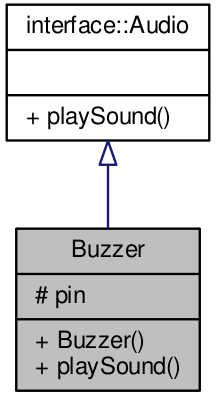
\includegraphics[scale=.35]{img/UML/CollaborationDiagram/Buzzer.png}
	\caption{Collaboration Diagram - Buzzer}
\end{figure}
\begin{figure}[!ht]
	\centering
	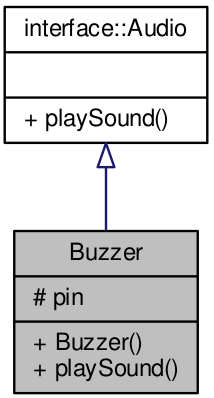
\includegraphics[scale=.35]{img/UML/InheritanceDiagram/Buzzer.png}
	\caption{Inheritance Diagram - Buzzer}
\end{figure}

\newpage
\subsection{Led.cpp, Led.h}
Classe per gestire l'accensione/spegnimento dei LED a 2 pin (controllo e massa) connessi all'Arduino.
\subsubsection{Metodi}
\begin{itemize}
	\item \texttt{protected	void switchOn()}: metodo che regola l'accensione istantanea del LED;
	\item \texttt{protected	void switchOff()}: metodo che regola lo spegnimento istantaneo del LED;
\end{itemize}
\begin{figure}[!ht]
	\centering
	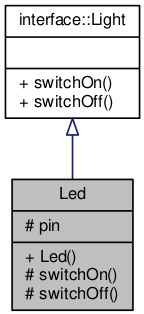
\includegraphics[scale=.5]{img/UML/CollaborationDiagram/Led.png}
	\caption{Collaboration Diagram - Led}
\end{figure}
\begin{figure}[!ht]
	\centering
	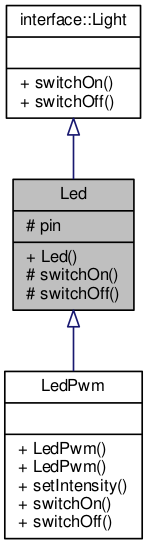
\includegraphics[scale=.5]{img/UML/InheritanceDiagram/Led.png}
	\caption{Inheritance Diagram - Led}
\end{figure}

\newpage
\subsection{LedPwm.cpp, LedPwm.h}
Questa classe permette l'accensione/spegnimento e dimmeraggio dei LED connessi ai pin PWM di Arduino
\subsubsection{Metodi}
\begin{itemize}
	\item \texttt{public void setIntensity(uint8\_t)}: imposta l'intensità luminosa emessa dal LED (compresa tra 0 e 255);
	\item \texttt{public void switchOn()}: imposta l'accensione istantanea del LED;
	\item \texttt{public void switchOff()}: imposta lo spegnimento istantaneo del LED;
\end{itemize}
\begin{figure}[!ht]
	\centering
	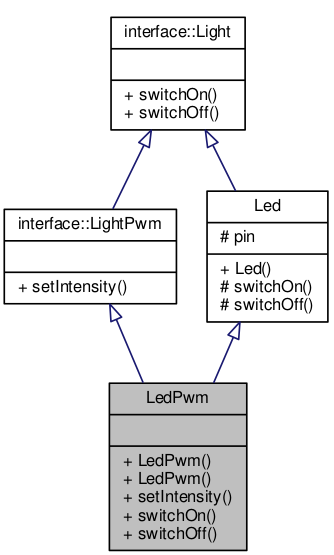
\includegraphics[scale=.4]{img/UML/CollaborationDiagram/LedPwm.png}
	\caption{Collaboration Diagram - LedPwm}
\end{figure}
\begin{figure}[!ht]
	\centering
	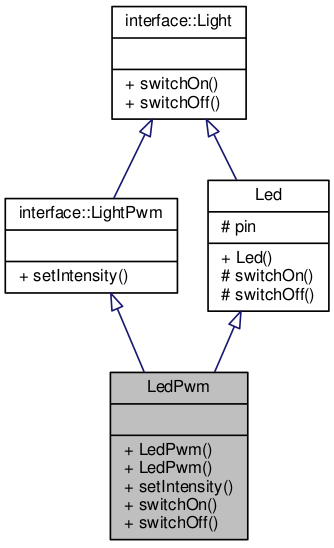
\includegraphics[scale=.4]{img/UML/InheritanceDiagram/LedPwm.png}
	\caption{Inheritance Diagram - LedPwm}
\end{figure}

\newpage
\subsection{LedRgb.cpp, LedRgb.h}
Questa classe permette il controllo dei LED RGB impostando i corretti pin per visualizzare il colore desiderato.

Nel dettaglio, il controllo viene eseguito istanziando tre oggetti \texttt{LedPwm} legati ad ogni colore/pin.
\subsubsection{Metodi}
\begin{itemize}
	\item \texttt{public void setColor(int, int, int)}: setta il colore da far vedere al giocatore;
	\item \texttt{protected	void switchOn()} : accensione istantanea del LED RGB;
	\item \texttt{protected	void switchOff()}: spegnimento istantaneo del LED RGB.
\end{itemize}
\begin{figure}[!ht]
	\centering
	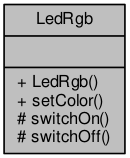
\includegraphics[scale=.5]{img/UML/CollaborationDiagram/LedRgb.png}
	\caption{Collaboration Diagram - LedRgb}
\end{figure}

\newpage
\subsection{Multiplexer.cpp, Multiplexer.h}
Classe che permette di gestire il multiplexer e quindi le sue uscite digitali. In questo progetto il multiplexer è strettamente legato ai LED a 12 pin regolando l'accensione/spegnimento di ogni LED interno. La classe è impostate per utilizzare la tabella di verità del multiplexer CD4067B.
\subsubsection{Metodi}
\begin{itemize}
	\item \texttt{public void switchOn(int)}: abilita il pin in uscita del multiplexer. Nel progetto è stato utile per visualizzare il livello a cui si sta giocando o il carosello sui LED a 12 pin;
	\item \texttt{public void carouselYellow(int)}: carosello del LED a 12 pin giallo, cioè si illuminano uno alla volta i LED interni per il periodo passato come intero;
	\item \texttt{public void carouselRed(int)}: carosello del LED a 12 pin rosso, con funzionamento identico al \texttt{carouselYellow(int)}.
\end{itemize}
\begin{figure}[!ht]
	\centering
	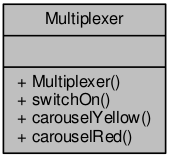
\includegraphics[scale=.5]{img/UML/CollaborationDiagram/Multiplexer.png}
	\caption{Collaboration Diagram - Multiplexer}
\end{figure}

\newpage
\subsection{MessageService.cpp, MessageService.h}
Questa classe permette di gestire l'invio e la ricezione di messaggi formattati in JSON attraverso la seriale.
Per codificare/decodificare i messaggi JSON è stata utilizzata la libreria \href{https://github.com/bblanchon/ArduinoJson}{ArduinoJson}\ref{sec:arduinojason}, facilitando le operazioni di I/O su seriale.
\subsubsection{Metodi}
\begin{itemize}
	\item \texttt{public void init(const int, const String \&)}: inizializza la seriale e stampa un messaggio di inizalizzazione;
	\item \texttt{public void setMessage(String)}  quando un messaggio viene letto, è parsato, se valido viene inviato un \textit{ACK};
	\item \texttt{public void errorMsg()}: invia un messaggio di errore;
	\item \texttt{public void ackMsg(const String)} : invio di un \textit{ACK};
	\item \texttt{public void sendMsg(const String, const String)}: invia un messaggio al destinatario.
	\item \texttt{public void sendInfo(const int, const int, const uint8\_t, const String)}: invia un messagio di servizio utile all'aggiornamento dello stato della partita.
\end{itemize}
\begin{figure}[!ht]
	\centering
	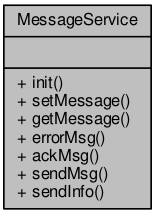
\includegraphics[scale=.5]{img/UML/CollaborationDiagram/MessageService.png}
	\caption{Collaboration Diagram - MessageService}
\end{figure}

\newpage
\section{Coordinamento dei task}
\section{Scheduler}
Lo Scheduler coordina l'esecuzione dei task secondo una schedulazione round-robin.

Al suo interno è presente un array \texttt{taskList} che contiene tutti i task da eseguire (aggiunti tramite \texttt{bool addTask(Task* task)}.

Nel caso in cui non ci siano task da eseguire o fossero tutti disabilitati, il sistema rimarrebbe apparentemente fermo (anche se in realtà il microcontrollore continuerebbe ad eseguire il suo \texttt{void loop()}).

Lo Scheduler è \textbf{cooperativo} in quanto una volta selezionato un task, questo viene eseguito fino al suo completamento (\textit{run-to-completion}).

Lo scheduling è a \textbf{priorità statica}, in quanto ad ogni task viene assegnata una priorità che non cambia durante l'esecuzione. La si può considerare come definita implicitamente dall'ordine di inserimento dei task nella \textit{task list}.

\section{Context.h}\label{sec:contextimpl}
La classe Context contiene tutti le variabili di stato del programma. I metodi al suo interno sono accessibili da tutti i task in modo da far evolvere il sistema; di seguito la lista di tutti i metodi e del loro significato.
\subsubsection{Metodi}
\begin{itemize}
	\item \texttt{bool isPadlockOpen(}): serve a sapere se il giocatore ha aperto il lucchetto;
	\item \texttt{void setPadlockOpen(bool padlockOpen)}: setting dello stato del lucchetto aperto/chiuso;
	\item \texttt{bool isPadlockDetected()}: serve a sapere se il giocatore ha trovato la giusta posizione del pistoncino;
	\item \texttt{void setPadlockDetected(bool padlockDetected)}: set dello stato del pistoncino trovato o no;
	\item \texttt{void setCurrentDistance(int currentDistance)}: set della distanza del padlock da aprire;
	\item \texttt{int getCurrentDistance()}: restituisce la distanza a cui si trova la mano;
	\item \texttt{void setButtonPressed(bool buttonPressed)}: set dello stato del bottone, se premuto o no;
	\item \texttt{ bool isButtonPressed()}: restituisce lo stato del bottone;
	\item \texttt{void setNewLevel()}: crea il nuovo livello da giocare;
	\item \texttt{uint8\_t getDelta()}: margine di errore della posizione del pistoncino;
	\item \texttt{uint8\_t getLevel()}: restituisce il livello attuale;
	\item \texttt{int getSecret()}: restituisce la distanza a cui si trova il lucchetto;
	\item \texttt{void newRandomNumber(}): genera un nuovo numero random;
	\item \texttt{void setGameOver(bool gameOver)}: setta lo stato del gioco, cioè se è finito o no;
	\item \texttt{bool isGameOver()}: restituisce lo stato del gioco, finito o no;
	\item \texttt{void setDangerLevel (uint8\_t dangerLevel)}:  set del livello di pericolo nello stato di scasso;
	\item \texttt{uint8\_t getDangerLevel()}: restituisce il livello di pericolo nello stato di scasso;
	\item \texttt{void setLockpicking (bool state)}: set dello stato di scasso;
	\item \texttt{bool isLockpicking()}: indica se ci si trova nello stato di scasso;
	\item \texttt{void carousel(uint8\_t delay1, uint8\_t delay2)}: esegue un carosello temporizzato dei due LED a 12 pin.
\end{itemize}
\begin{figure}[!ht]
	\centering
	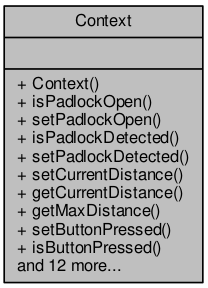
\includegraphics[scale=.5]{img/UML/CollaborationDiagram/Context.png}
	\caption{Collaboration Diagram - Context}
\end{figure}

\newpage
\subsection{Scheduler.cpp, Scheduler.h}
\subsubsection{Metodi}
\begin{itemize}
	\item \texttt{public void init(int)}: inizializza il base period dello Scheduler;
	\item \texttt{public virtual bool addTask(Task *)}: aggiunge il task alla lista dei task da eseguire;
	\item \texttt{public virtual void schedule()}: pianifica l'esecuzione dei vari task, eseguendoli uno alla volta. Nel caso in cui un task non sia abilitato, viene semplicemente ignorato (non eseguendo il suo tick) e quindi si passa immediatamente al successivo della lista.
\end{itemize}
\begin{figure}[!ht]
	\centering
	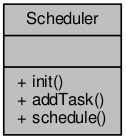
\includegraphics[scale=.5]{img/UML/CollaborationDiagram/Scheduler.png}
	\caption{Collaboration Diagram - Scheduler}
\end{figure}

\subsection{Timer.h, Timer.cpp}
\subsubsection{Metodi}
\begin{itemize}
	\item public void setupPeriod(int): disabilita gli \textit{interrupt}, setta i registri del Timer1 (configurando il prescale) e riabilita gli interrupt;
	\item public void waitForNextTick(): permette di eseguire il task.
\end{itemize}
\begin{figure}[!ht]
	\centering
	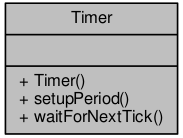
\includegraphics[scale=.5]{img/UML/CollaborationDiagram/Timer.png}
	\caption{Collaboration Diagram - Timer}
\end{figure}

\newpage
\subsection{Task.h}
\subsubsection{Metodi}
\begin{figure}[!ht]
	\centering
	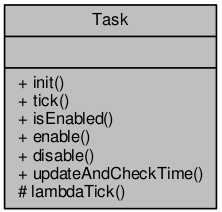
\includegraphics[scale=.5]{img/UML/CollaborationDiagram/Task.png}
	\caption{Collaboration Diagram - Task}
\end{figure}
\begin{figure}[!ht]
	\centering
	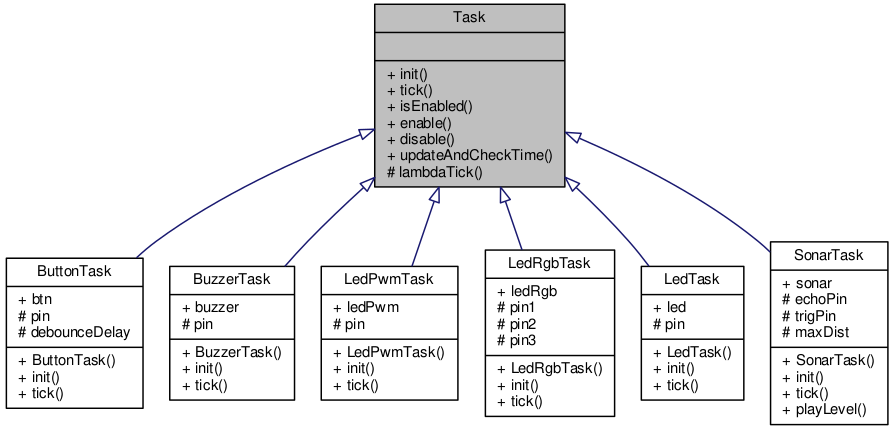
\includegraphics[scale=.35]{img/UML/InheritanceDiagram/Task.png}
	\caption{Inheritance Diagram - Task}
\end{figure}